\chapter{Implementasi dan Pengujian}
\label{chap: implemenPengujian}

Pada bagian ini merupakan rincian atau penjelasan lanjut mengenai lingkungan implementasi perangkat keras maupun perangkat lunak sistem informasi penilaian sidang skripsi 2. Bagian terakhir akan membahas tentang pengujian yang telah dilakukan pada sistem informasi.

\section{Implementasi}
\label{sec: implementasi}

	Pada bagian ini akan dijabarkan lingkungan pengembangan sistem informasi dan pengujian.
	
	\subsection{Lingkungan Implementasi dan Pengujian}
	\label{sub: lingkunganImp}
	
	Implementasi dilakukan dengan menggunakan sebuah laptop. Berikut adalah spesifikasi laptop
	yang digunakan:
	
	\begin{enumerate}
		\item Processor: Intel(R) Core(TM) i7-6500U CPU @ 2.50GHz (4 CPUs), ~2.6GHz
		\item RAM : 4096 MB
		\item Sistem operasi : Windows 10 Home Single Language 64-bit (10.0, Build 14393)
		\item Versi AngularJS : Version 1.5.2
		\item Versi Codeigniter : Version 3.1.3
		\item Versi TwitterBootstrap : Version 2.3.2
		\item Versi Google Chrome : Version 57.0.2987.133 (64-bit)
	\end{enumerate}

	\subsection{Hasil Implementasi}
	\label{sub: hasilImplemen}
	
	Hasil implementasi dari penelitian ini adalah sebuah sistem informasi berbasis web yang menggunakan \textit{codeigniter}, \textit{AngularJS}, dan \textit{Twitter Bootstrap} sebagai dasar pembuatan. Aplikasi dapat diakses melalui jaringan \textit{global} dengan URL \url{http://sipskripsi.com}. Sistem informasi terdiri dari bagian-bagian sebagai berikut:
	
	\begin{itemize}
		\item Bagian formulir berita acara sidang skripsi\\
		Bagian ini adalah halaman yang bersangkutan dalam pengisian data diri mahasiswa yang bersangkutan, sekaligus sebagai halaman akhir yang menyimpulkan perhitungan nilai akhir mahasiswa. Kolom penilaian pada halaman ini tidak dapat diisi secara manual kecuali kolom penilaian milik koordinator skripsi. Kolom penilaian yang lain didapatkan berdasarkan perhitungan nilai akhir masing-masing penguji.
		\begin{figure}[H]
			\centering
			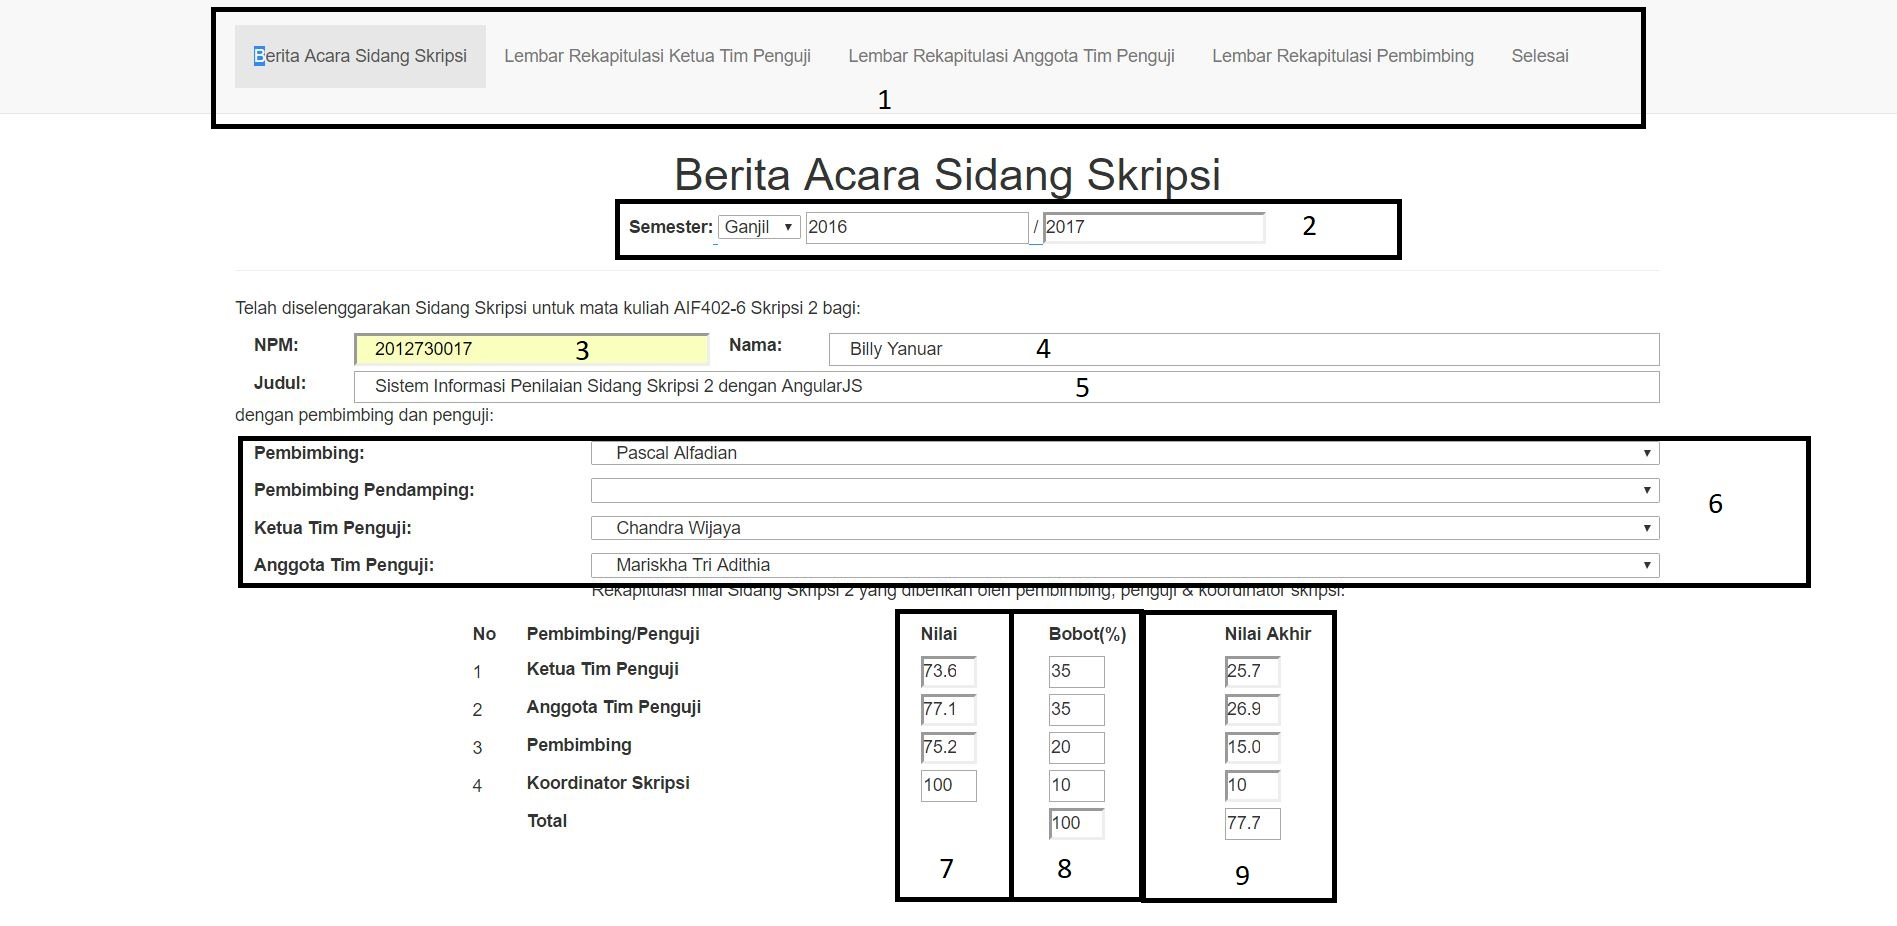
\includegraphics[scale=0.4]{Gambar/beritaacaraisi}
			\caption{Formulir berita acara sidang skripsi 2 terisi}
			\label{fig:beritaisi}
		\end{figure}
	Keterangan Gambar \ref{fig:beritaisi}.
		\begin{enumerate}
			\item Tempat navigasi untuk berpindah halaman
			\item Pengisian semester sidang (Genap/Ganjil), dan tahun sidang (default 2016 / otomatis +1)
			\item NPM mahasiswa (harus tepat 10 angka)
			\item Nama mahasiswa
			\item Judul skripsi
			\item Data diri penilai (nama ketua tim penguji, anggota tim penguji, pembimbing, dan pembimbing pendamping)
			\item Kotak masukan nilai per kategori (otomatis diambil dari rekapitulasi)
			\item Bobot nilai yang dimiliki kategori (\textit{default})
			\item Nilai hasil perhitungan nilai dengan bobot (otomatis)
		\end{enumerate}
		\item Bagian formulir rekapitulasi penilaian sidang skripsi 2.\\
		Bagian ini adalah halaman yang bersangkutan dalam menampung nilai-nilai yang diberikan oleh ketua tim penguji, anggota tim penguji, dan pembimbing pada mahasiswa. 
		\begin{figure}[H]
			\centering
			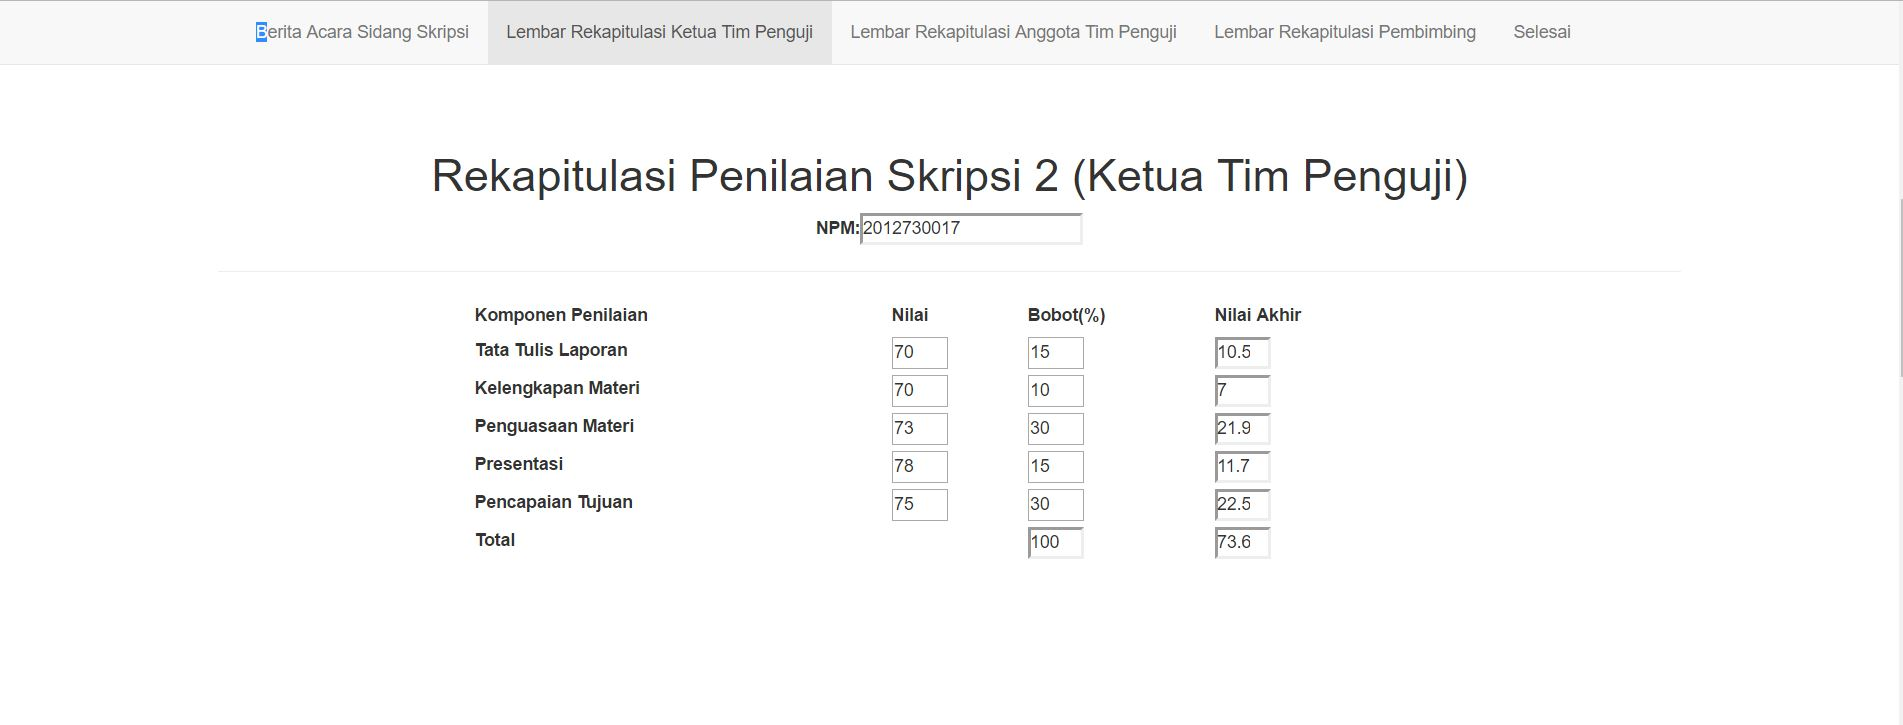
\includegraphics[scale=0.4]{Gambar/ketuaisi}
			\caption{Formulir rekapitulasi ketua tim penguji terisi}
			\label{fig:ketuaisi}
		\end{figure}
	Keterangan Gambar \ref{fig:ketuaisi}.
	\begin{enumerate}
		\item Tempat navigasi untuk berpindah halaman
		\item NPM mahasiswa (otomatis diambil dari berita acara)
		\item Kotak masukan nilai per kategori (masukan)
		\item Bobot nilai yang dimiliki kategori (\textit{default})
		\item Nilai hasil perhitungan nilai dengan bobot (otomatis)
	\end{enumerate}
		\begin{figure}[H]
			\centering
			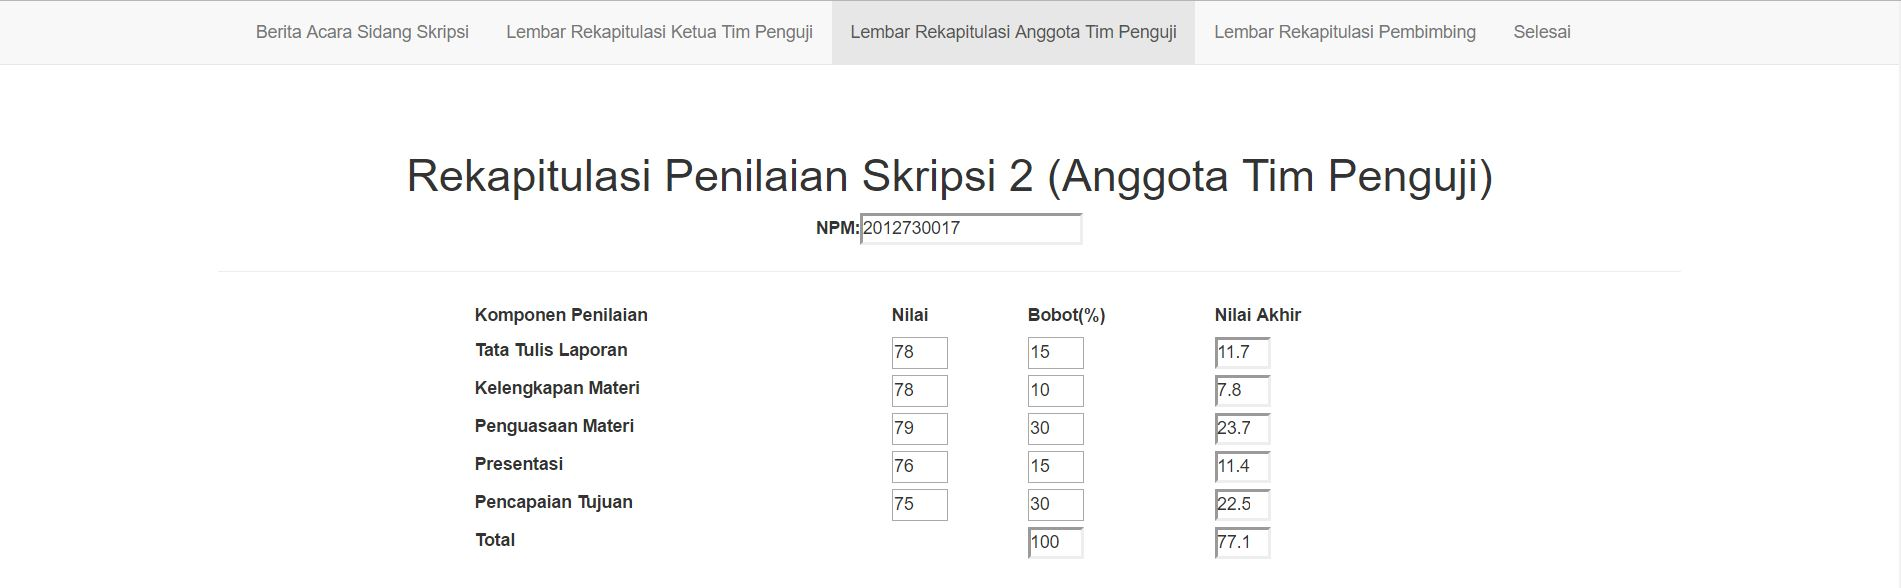
\includegraphics[scale=0.4]{Gambar/anggotaisi}
			\caption{Formulir rekapitulasi anggota tim penguji terisi}
			\label{fig:anggotaisi}
		\end{figure}
	Keterangan Gambar \ref{fig:anggotaisi}.
	\begin{enumerate}
		\item Tempat navigasi untuk berpindah halaman
		\item NPM mahasiswa (otomatis diambil dari berita acara)
		\item Kotak masukan nilai per kategori (masukan)
		\item Bobot nilai yang dimiliki kategori (\textit{default})
		\item Nilai hasil perhitungan nilai dengan bobot (otomatis)
	\end{enumerate}
		\begin{figure}[H]
			\centering
			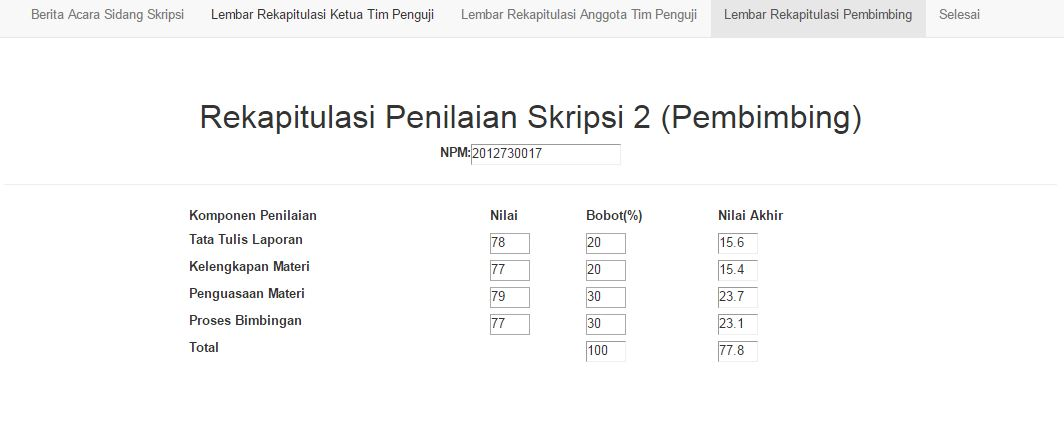
\includegraphics[scale=0.4]{Gambar/pembimbingisi}
			\caption{Formulir rekapitulasi pembimbing terisi}
			\label{fig:pembimbingisi}
		\end{figure}
	Keterangan Gambar \ref{fig:ketuaisi}.
	\begin{enumerate}
		\item Tempat navigasi untuk berpindah halaman
		\item NPM mahasiswa (otomatis diambil dari berita acara)
		\item Kotak masukan nilai per kategori (masukan)
		\item Bobot nilai yang dimiliki kategori (\textit{default})
		\item Nilai hasil perhitungan nilai dengan bobot (otomatis)
	\end{enumerate}
		\item Bagian selesai.\\
		Bagian ini adalah bagian terakhir dari sistem informasi. Ketika formulir sudah selesai diisi, diperlukan persetujuan dengan cara menandai checkbox dari 3 pihak penilai yaitu ketua tim penguji, anggota tim penguji, dan pembimbing. Setelah selesai, dengan menekan tombol selesai pada bagian ini, akan terdapat sebuah pop up untuk memastikan bahwa pengisian sistem telah selesai. Jika "OK" d tekan, maka \textit{data} yang telah terisi akan dimasukkan ke dalam \textit{database}.
		\begin{figure}[H]
			\centering
			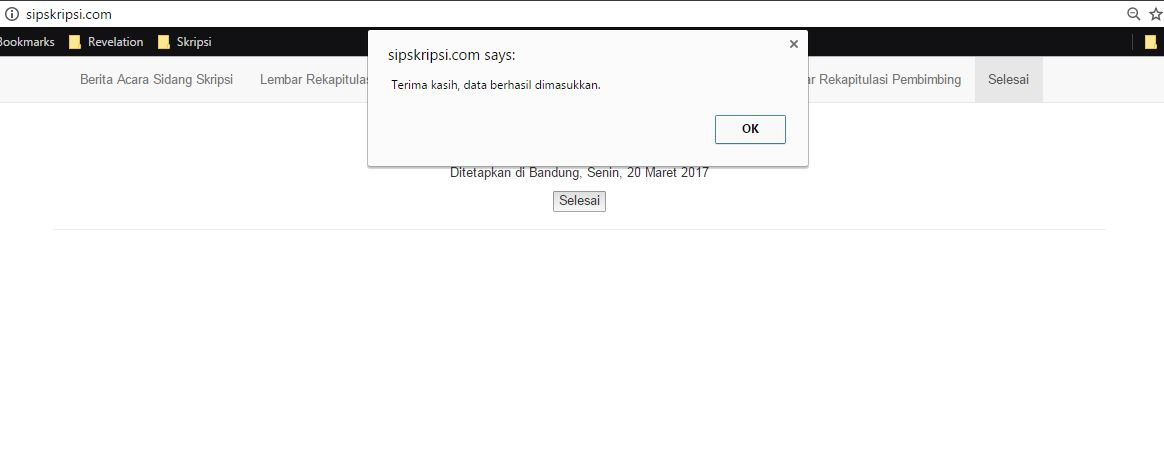
\includegraphics[scale=0.4]{Gambar/selesaiisi}
			\caption{Pengisian Checkbox}
			\label{tab: hasilPeng}
		\end{figure}
	\begin{figure}[H]
		\centering
		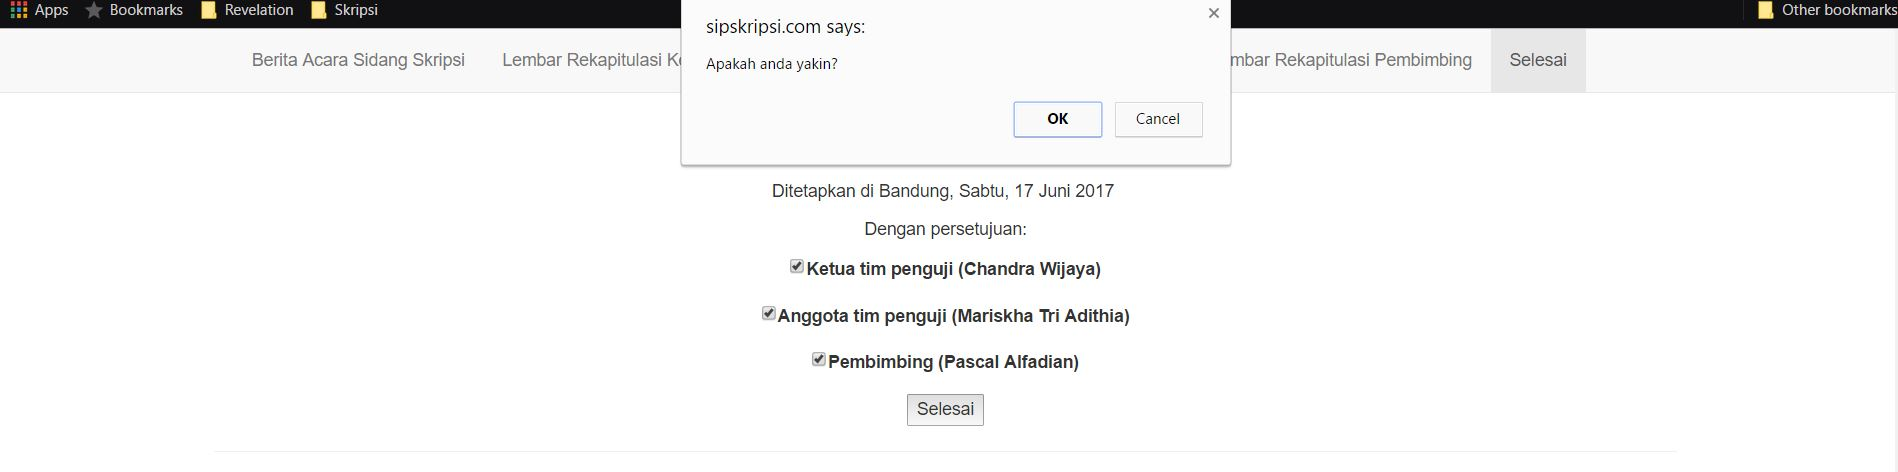
\includegraphics[scale=0.4]{Gambar/selesaiisi2}
		\caption{Pop Up untuk memastikan pengisian nilai sistem}
		\label{tab: hasilPeng2}
	\end{figure}
		\begin{table}[htbp]
			\centering
			\caption{Tabel Hasil Implementasi}
			\begin{tabular}{| m{7cm} | m{5cm} |}
				\hline
				Jenis Data & Input Nilai\\
				\hline
				id & 32\\
				\hline
				tahun & 2017\\
				\hline
				semester & 2\\
				\hline
				npm & 2012730017\\
				\hline
				nama & Billy Yanuar\\
				\hline
				judul & Sistem Informasi Penilaian Sidang Skripsi 2 dengan AngularJS\\
				\hline
				namaPembimbing & Pascal Alfadian\\
				\hline
				namaPembimbingPendamping & \\
				\hline
				namaKetuaTimPenguji & Chandra Wijaya\\
				\hline
				namaAnggotaTimPenguji & Mariskha Tri Adithia\\
				\hline
				bobotKetuaTimPenguji & 35\\
				\hline
				bobotAnggotaTimPenguji & 35\\
				\hline
				bobotPembimbing & 20\\
				\hline
				nilaiKoordinatorSkripsi & 100\\
				\hline
				bobotKoordinatorSkripsi & 10\\
				\hline
				bobotTataTulisLaporanAnggota & 15\\
				\hline
				bobotKelengkapanMateriAnggota & 10\\
				\hline
				bobotPenguasaanMateriAnggota & 30\\
				\hline
				bobotPresentasiAnggota & 15\\
				\hline
				bobotPencapaianTujuanKetua & 30\\
				\hline
				bobotTataTulisLaporanKetua & 15\\
				\hline
				bobotKelengkapanMateriKetua & 10\\
				\hline
				bobotPenguasaanMateriKetua & 30\\
				\hline
				bobotPresentasiKetua & 15\\
				\hline
				bobotPencapaianTujuanKetua & 30\\
				\hline
				bobotTataTulisLaporanPembimbing & 20\\
				\hline
				bobotKelengkapanMateriPembimbing &20\\
				\hline
				bobotPenguasaanMateriPembimbing & 30\\
				\hline
				prosesBimbinganPembimbing & 30\\
				\hline
				nilaiAkhirMahasiswa & 77.785\\
				\hline
			\end{tabular}
		\end{table}
	\end{itemize}
	
\section{Hasil Pengujian}
\label{sec:hasilUji}

	Pengujian pada sistem informasi penilaian sidang skripsi 2 merupakan pengujian bersifat fungsional, dan pengujian eksperimental. Berikut penjelasannya:
	
	\subsection{Pengujian Fungsional}
	\label{sub: PFungsional}
	
	Pengujian eksperimental dilakukan dengan cara mengikuti sidang Skripsi 2 yang dilakukan pada semester ganjil 2016/2017. Pada sidang yang diujikan, penilaian dilakukan dengan dua cara, yaitu dengan sistem kini yang bekerja secara manual dan dengan sistem usulan menggunakan laptop. Sehubungan dengan sifat kerasahasiaan \textit{data} pengujian, maka dengan persetujuan pembimbing pengujian eksperimental dilakukan dengan merahasiakan identitas mahasiswa yang berhubungan.
	
	Pada saat melakukan pengujian eksperimental, sistem kini memiliki kekurangan kecerobohan manusia yang mengakibatkan kesalahan dalam perhitungan nilai baik dari lembar rekapitulasi maupun lembar berita acara sidang skripsi. Hal tersebut diketahui pada saat membandingkan nilai perhitungan nilai akhir yang didapatkan oleh mahasiswa pada sistem kini dan sistem usulan. Pada beberapa kesalahan tersebut, penguji kembali melakukan perhitungan secara manual dengan menggunakan mesin hitung berupa kalkulator pada \textit{gadget} penguji. Setelah perhitungan dilakukan, didapatkan bahwa sistem usulan memiliki hasil yang benar.
	
	Percobaan eksperimental menghasilkan kesimpulan sistem usulan dapat menutupi kekurangan sistem kini yang berfokus pada perhitungan penilaian mahasiswa. Dengan menggunakan sistem usulan, perhitungan nilai dibuktikan lebih akurat dibandingkan dengan sistem kini. Berikut ini adalah hasil dari pengujian eksperimental.
	\begin{table}[H]
		\centering
		\caption{Tabel Pengujian Eksperimental 1}
		\begin{tabular}{| m{7cm} | m{5cm} |}
			\hline
			Jenis Data & Input Nilai\\
			\hline
			id & 26\\
			\hline
			tahun & 2016\\
			\hline
			semester & 1\\
			\hline
			npm & 2012730001\\
			\hline
			nama & A\\
			\hline
			judul & Tidak Dicatat \\
			\hline
			namaPembimbing & Mariskha A\\
			\hline
			namaPembimbingPendamping & -\\
			\hline
			namaKetuaTimPenguji & Pascal A\\
			\hline
			namaAnggotaTimPenguji & Joanna H\\
			\hline
			bobotKetuaTimPenguji & 35\\
			\hline
			bobotAnggotaTimPenguji & 35\\
			\hline
			bobotPembimbing & 20\\
			\hline
		\end{tabular}
	\end{table}
	\begin{table}[H]
	\centering
		\begin{tabular}{| m{7cm} | m{5cm} |}
		\hline
			nilaiKoordinatorSkripsi & 100\\
			\hline
			bobotKoordinatorSkripsi & 10\\
			\hline
			bobotTataTulisLaporanAnggota & 15\\
			\hline
			bobotKelengkapanMateriAnggota & 10\\
			\hline
			bobotPenguasaanMateriAnggota & 30\\
			\hline
			bobotPresentasiAnggota & 15\\
			\hline
			bobotPencapaianTujuanKetua & 30\\
			\hline
			bobotTataTulisLaporanKetua & 15\\
			\hline
			bobotKelengkapanMateriKetua & 10\\
			\hline
			bobotPenguasaanMateriKetua & 30\\
			\hline
			bobotPresentasiKetua & 15\\
			\hline
			bobotPencapaianTujuanKetua & 30\\
			\hline
			bobotTataTulisLaporanPembimbing & 20\\
			\hline
			bobotKelengkapanMateriPembimbing &20\\
			\hline
			bobotPenguasaanMateriPembimbing & 30\\
			\hline
			prosesBimbinganPembimbing & 30\\
			\hline
			nilaiAkhirMahasiswa & 83\\
			\hline
		\end{tabular}
	\end{table}
	\begin{table}[H]
		\centering
		\caption{Tabel Pengujian Eksperimental 2}
		\begin{tabular}{| m{7cm} | m{5cm} |}
			\hline
			Jenis Data & Input Nilai\\
			\hline
			id & 27\\
			\hline
			tahun & 2016\\
			\hline
			semester & 1\\
			\hline
			npm & 2012730002\\
			\hline
			nama & B\\
			\hline
			judul & Tidak Dicatat \\
			\hline
			namaPembimbing & Luciana A\\
			\hline
			namaPembimbingPendamping & -\\
			\hline
			namaKetuaTimPenguji & Cecilian E N\\
			\hline
			namaAnggotaTimPenguji & Vania\\
			\hline
			bobotKetuaTimPenguji & 35\\
			\hline
			bobotAnggotaTimPenguji & 35\\
			\hline
			bobotPembimbing & 20\\
			\hline
			nilaiKoordinatorSkripsi & 100\\
			\hline
			bobotKoordinatorSkripsi & 10\\
			\hline
			bobotTataTulisLaporanAnggota & 15\\
			\hline
			bobotKelengkapanMateriAnggota & 10\\
			\hline
			bobotPenguasaanMateriAnggota & 30\\
			\hline
			bobotPresentasiAnggota & 15\\
			\hline
			bobotPencapaianTujuanKetua & 30\\
			\hline
			bobotTataTulisLaporanKetua & 15\\
			\hline
			bobotKelengkapanMateriKetua & 10\\
			\hline
			bobotPenguasaanMateriKetua & 30\\
			\hline
			bobotPresentasiKetua & 15\\
			\hline
			bobotPencapaianTujuanKetua & 30\\
			\hline
			bobotTataTulisLaporanPembimbing & 20\\
			\hline
			bobotKelengkapanMateriPembimbing &20\\
			\hline
			bobotPenguasaanMateriPembimbing & 30\\
			\hline
			prosesBimbinganPembimbing & 30\\
			\hline
			nilaiAkhirMahasiswa & 84\\
			\hline
		\end{tabular}
	\end{table}
	\begin{table}[H]
		\centering
		\caption{Tabel Pengujian Eksperimental 3}
		\begin{tabular}{| m{7cm} | m{5cm} |}
			\hline
			Jenis Data & Input Nilai\\
			\hline
			id & 28\\
			\hline
			tahun & 2016\\
			\hline
			semester & 1\\
			\hline
			npm & 2012730003\\
			\hline
			nama & C\\
			\hline
			judul & Tidak Dicatat \\
			\hline
			namaPembimbing & Anoeng\\
			\hline
			namaPembimbingPendamping & -\\
			\hline
			namaKetuaTimPenguji & Bagoes\\
			\hline
			namaAnggotaTimPenguji & Pascal A\\
			\hline
			bobotKetuaTimPenguji & 35\\
			\hline
			bobotAnggotaTimPenguji & 35\\
			\hline
			bobotPembimbing & 20\\
			\hline
			nilaiKoordinatorSkripsi & 100\\
			\hline
			bobotKoordinatorSkripsi & 10\\
			\hline
			bobotTataTulisLaporanAnggota & 15\\
			\hline
			bobotKelengkapanMateriAnggota & 10\\
			\hline
			bobotPenguasaanMateriAnggota & 30\\
			\hline
			bobotPresentasiAnggota & 15\\
			\hline
			bobotPencapaianTujuanKetua & 30\\
			\hline
			bobotTataTulisLaporanKetua & 15\\
			\hline
			bobotKelengkapanMateriKetua & 10\\
			\hline
			bobotPenguasaanMateriKetua & 30\\
			\hline
			bobotPresentasiKetua & 15\\
			\hline
			bobotPencapaianTujuanKetua & 30\\
			\hline
			bobotTataTulisLaporanPembimbing & 20\\
			\hline
			bobotKelengkapanMateriPembimbing &20\\
			\hline
			bobotPenguasaanMateriPembimbing & 30\\
			\hline
			prosesBimbinganPembimbing & 30\\
			\hline
			nilaiAkhirMahasiswa & 76\\
			\hline
		\end{tabular}
	\end{table}
	\begin{table}[H]
		\centering
		\caption{Tabel Pengujian Eksperimental 4}
		\begin{tabular}{| m{7cm} | m{5cm} |}
			\hline
			Jenis Data & Input Nilai\\
			\hline
			id & 29\\
			\hline
			tahun & 2016\\
			\hline
			semester & 1\\
			\hline
			npm & 2012730004\\
			\hline
			nama & DE\\
			\hline
			judul & Tidak Dicatat \\
			\hline
			namaPembimbing & Pascal A\\
			\hline
			namaPembimbingPendamping & -\\
			\hline
			namaKetuaTimPenguji & Gede Karya\\
			\hline
			namaAnggotaTimPenguji & Rosa De Lima\\
			\hline
			bobotKetuaTimPenguji & 35\\
			\hline
			bobotAnggotaTimPenguji & 35\\
			\hline
		\end{tabular}
	\end{table}
\begin{table}[H]
\centering
\begin{tabular}{| m{7cm} | m{5cm} |}
\hline
			bobotPembimbing & 20\\
			\hline
			nilaiKoordinatorSkripsi & 100\\
			\hline
			bobotKoordinatorSkripsi & 10\\
			\hline
			bobotTataTulisLaporanAnggota & 15\\
			\hline
			bobotKelengkapanMateriAnggota & 10\\
			\hline
			bobotPenguasaanMateriAnggota & 30\\
			\hline
			bobotPresentasiAnggota & 15\\
			\hline
			bobotPencapaianTujuanKetua & 30\\
			\hline
			bobotTataTulisLaporanKetua & 15\\
			\hline
			bobotKelengkapanMateriKetua & 10\\
			\hline
			bobotPenguasaanMateriKetua & 30\\
			\hline
			bobotPresentasiKetua & 15\\
			\hline
			bobotPencapaianTujuanKetua & 30\\
			\hline
			bobotTataTulisLaporanPembimbing & 20\\
			\hline
			bobotKelengkapanMateriPembimbing &20\\
			\hline
			bobotPenguasaanMateriPembimbing & 30\\
			\hline
			prosesBimbinganPembimbing & 30\\
			\hline
			nilaiAkhirMahasiswa & 78\\
			\hline
		\end{tabular}
	\end{table}
	\begin{table}[H]
		\centering
		\caption{Tabel Pengujian Eksperimental 5}
		\begin{tabular}{| m{7cm} | m{5cm} |}
			\hline
			Jenis Data & Input Nilai\\
			\hline
			id & 30\\
			\hline
			tahun & 2016\\
			\hline
			semester & 1\\
			\hline
			npm & 2012730004\\
			\hline
			nama & E\\
			\hline
			judul & Tidak Dicatat\\
			\hline
			namaPembimbing & Mariskha A\\
			\hline
			namaPembimbingPendamping & -\\
			\hline
			namaKetuaTimPenguji & Husnul\\
			\hline
			namaAnggotaTimPenguji & Chandra\\
			\hline
			bobotKetuaTimPenguji & 35\\
			\hline
			bobotAnggotaTimPenguji & 35\\
			\hline
			bobotPembimbing & 20\\
			\hline
			nilaiKoordinatorSkripsi & 100\\
			\hline
			bobotKoordinatorSkripsi & 10\\
			\hline
			bobotTataTulisLaporanAnggota & 15\\
			\hline
			bobotKelengkapanMateriAnggota & 10\\
			\hline
			bobotPenguasaanMateriAnggota & 30\\
			\hline
			bobotPresentasiAnggota & 15\\
			\hline
			bobotPencapaianTujuanKetua & 30\\
			\hline
			bobotTataTulisLaporanKetua & 15\\
			\hline
			bobotKelengkapanMateriKetua & 10\\
			\hline
			bobotPenguasaanMateriKetua & 30\\
			\hline
			bobotPresentasiKetua & 15\\
			\hline
			bobotPencapaianTujuanKetua & 30\\
			\hline
			bobotTataTulisLaporanPembimbing & 20\\
			\hline
			bobotKelengkapanMateriPembimbing &20\\
			\hline
			bobotPenguasaanMateriPembimbing & 30\\
			\hline
			prosesBimbinganPembimbing & 30\\
			\hline
			nilaiAkhirMahasiswa & 84\\
			\hline
		\end{tabular}
	\end{table}

		Tabel \ref{pengFung} adalah hasil pengujian sistem usulan pada berbagai macam \textit{platform}, yang bertujuan untuk mengetahui apakah sistem informasi dapat menjalankan seluruh fungsi-fungsi yang dimiliki dengan baik ketika dijalankan pada \textit{platform} yang berbeda.
		
	\begin{table}[H]
		\centering
		\caption{Tabel Pengujian Fungsional}
		\label{pengFung}
		\begin{tabular}{| m{0.75cm} | m{7cm} | m{5cm} | m{3cm} |}
			\hline
			No & Aksi Pengguna & Reaksi yang diharapkan & Keterangan \\
			\hline
			1 & Pengguna menjalankan sistem informasi pada browser Microsoft Edge & Halaman ditampilkan dengan perbedaan tampilan pada tombol pengubah angka serta checklist & Fungsi berjalan sesuai \\
			\hline
			2 & Pengguna menjalankan sistem informasi pada browser Mozilla Firefox & Halaman ditampilkan dengan perbedaan tampilan pada tombol pengubah angka serta checklist & Fungsi berjalan sesuai \\
			\hline
			3 & Pengguna menjalankan sistem informasi pada mobile device berupa smartphone & Halaman ditampilkan dengan perbedaan pada tampilan & Fungsi berjalan sesuai \\
			\hline
		\end{tabular}
	\end{table}

\begin{figure}[H]
	\centering
	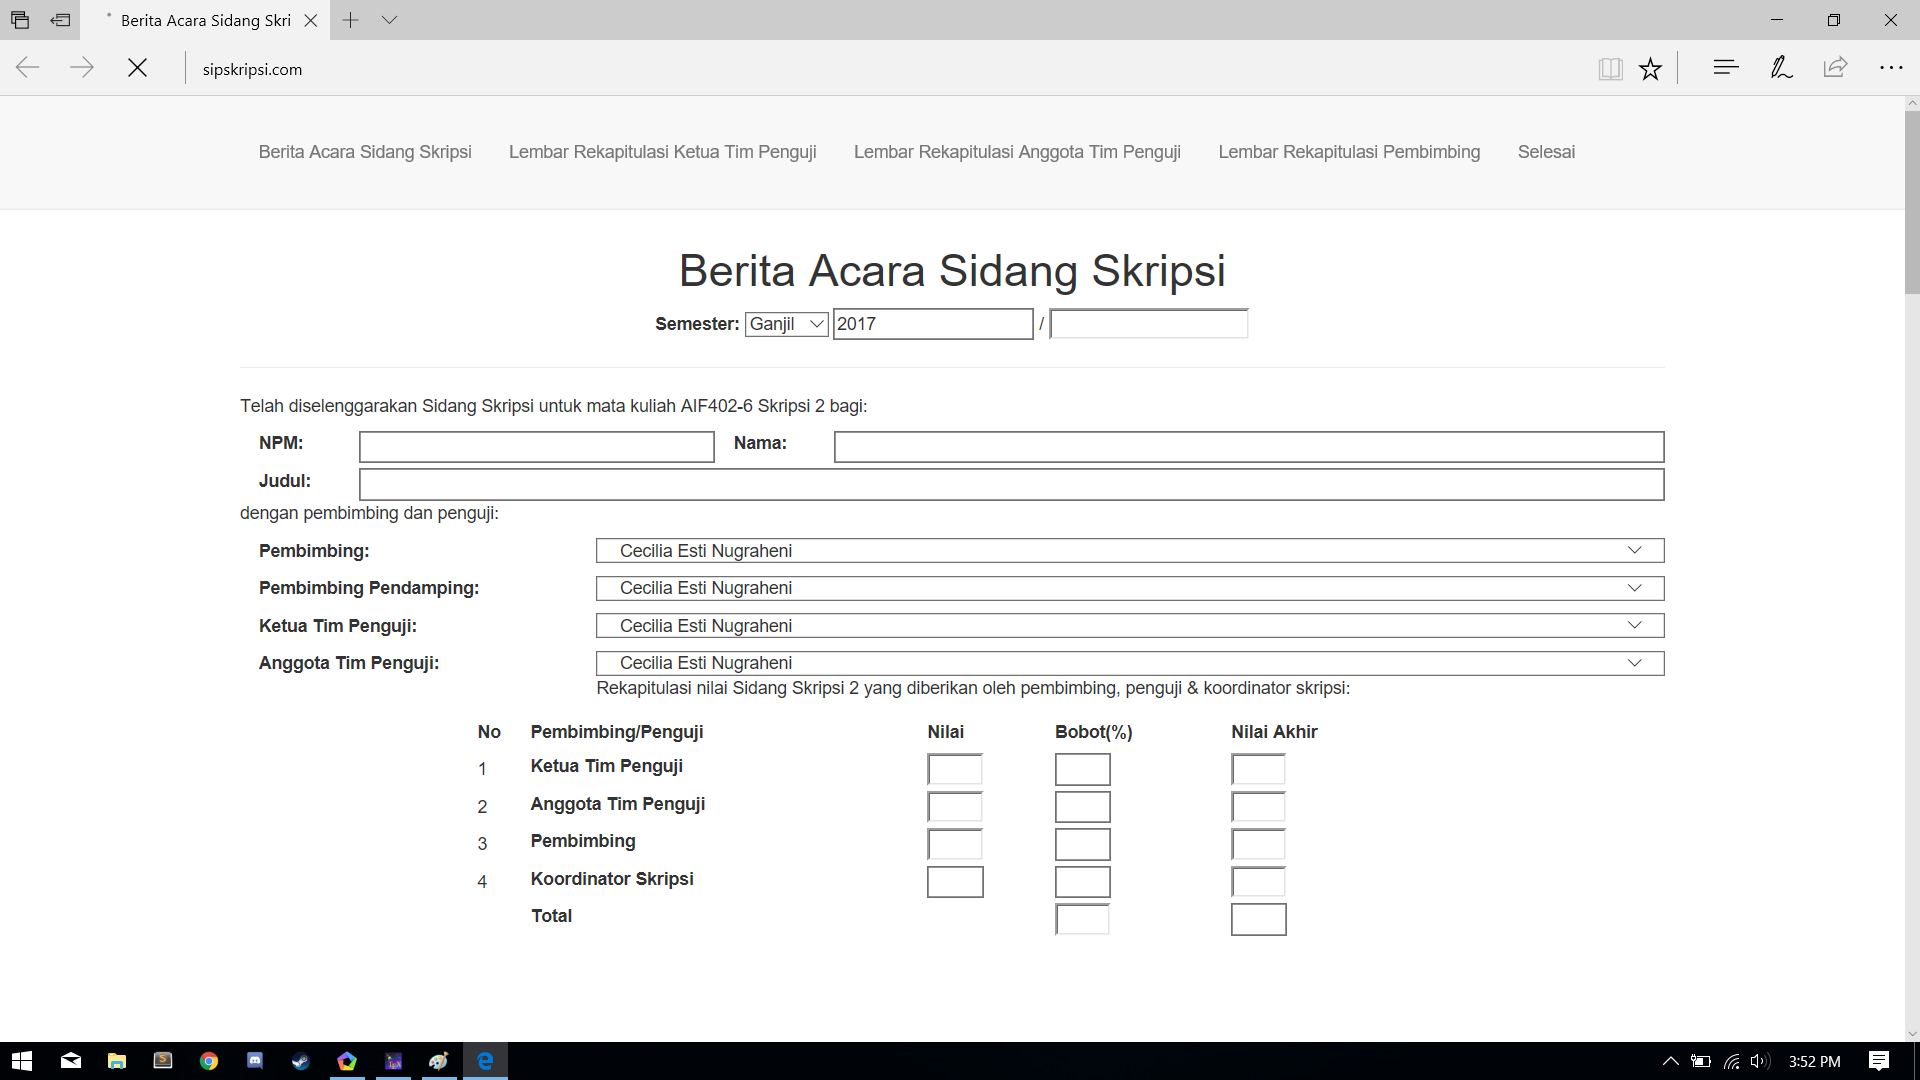
\includegraphics[scale=0.3]{Gambar/MsEdge}
	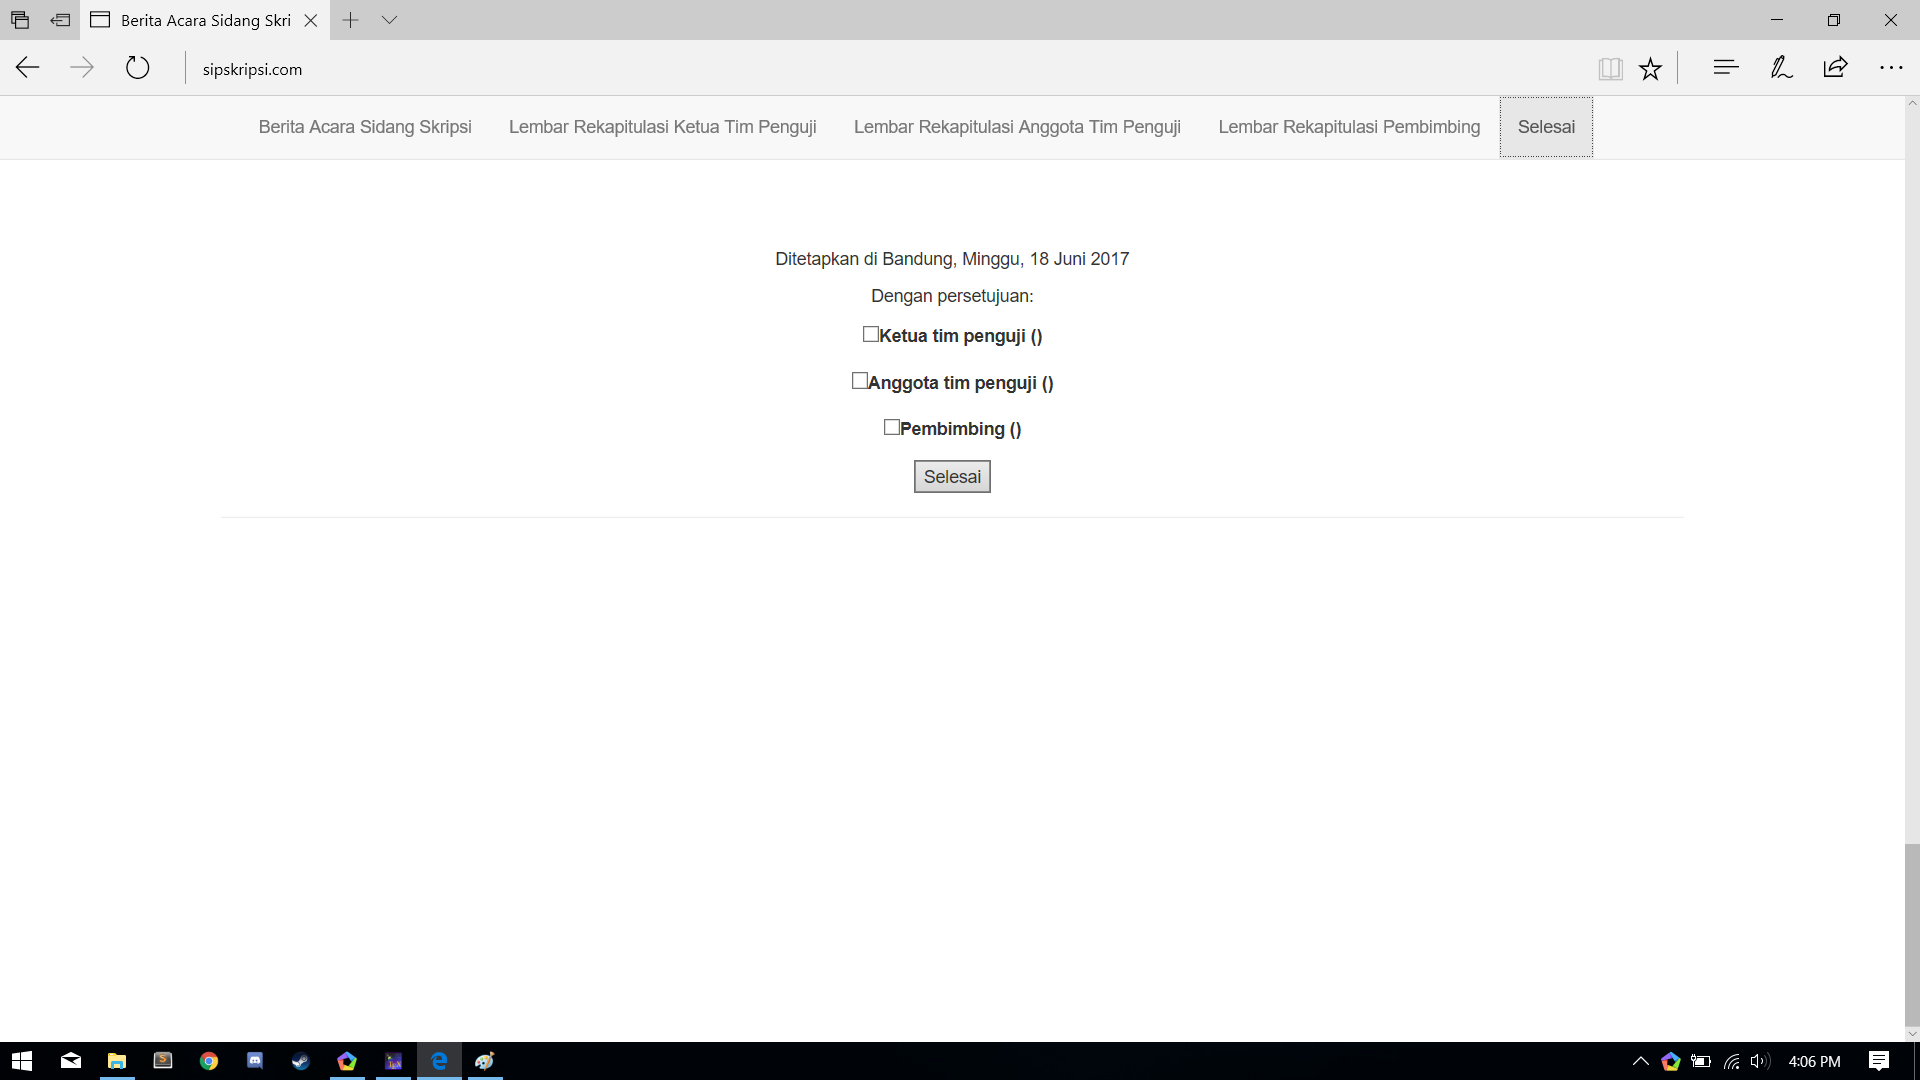
\includegraphics[scale=0.3]{Gambar/MsEdgeSelesai}
	\caption{Tampilan sistem pada platform Microsoft Edge}
	\label{fig:MsEdge}
\end{figure}

\begin{figure}[H]
	\centering
	\includegraphics[scale=0.4]{Gambar/Mozila}
	\includegraphics[scale=0.4]{Gambar/MozilaSelesai}
	\caption{Tampilan sistem pada platform Mozilla Firefox}
	\label{fig:Mozila}
\end{figure}

\begin{figure}[H]
	\centering
	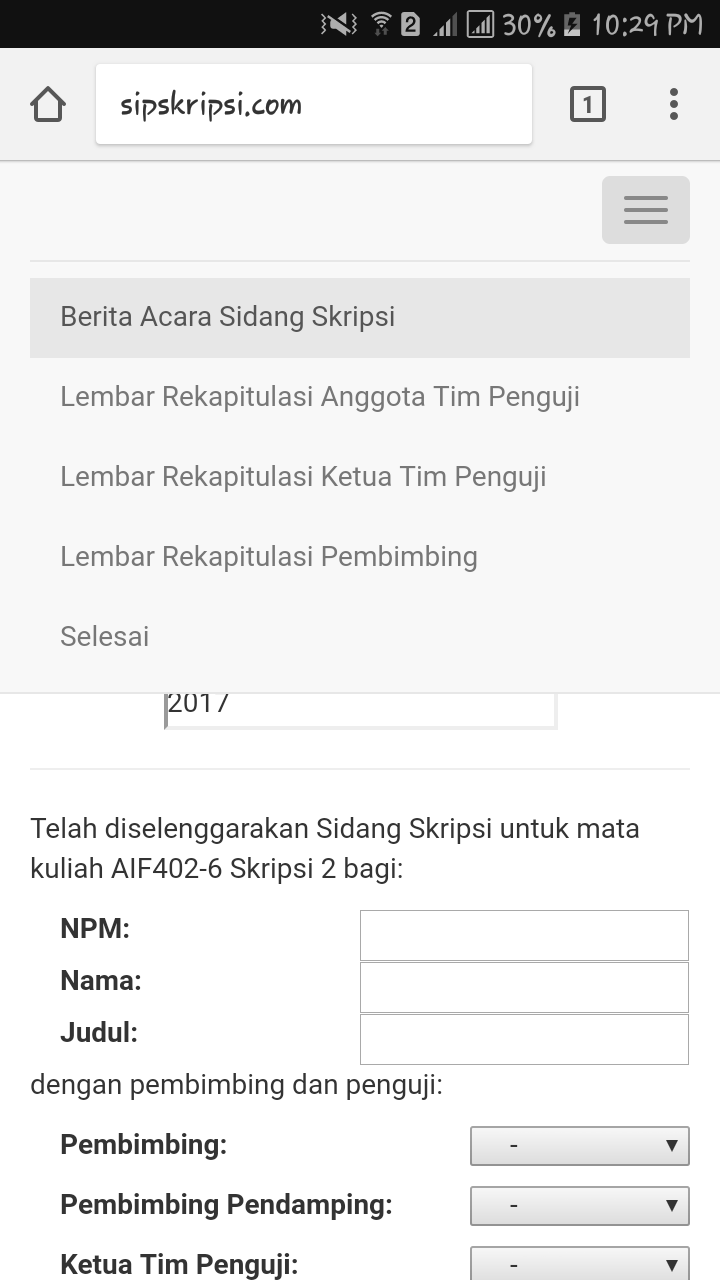
\includegraphics[scale=0.2]{Gambar/hp_menu}
	\caption{Tampilan menu sistem pada platform browser smartphone}
	\label{fig:hp_menu}
\end{figure}

\begin{figure}[H]
	\centering
	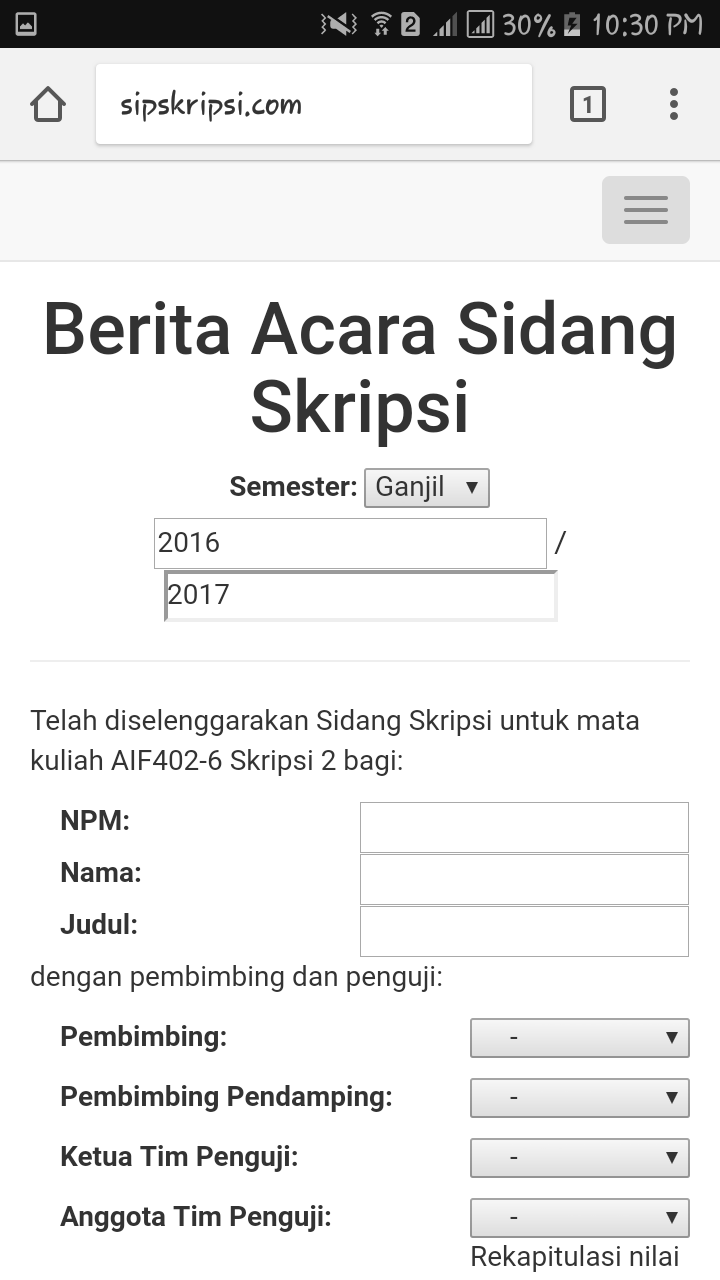
\includegraphics[scale=0.2]{Gambar/hp_beritaacara}
	\caption{Tampilan lembar berita acara sistem sidang skripsi pada platform browser smartphone}
	\label{fig:hp_beritaacara}
\end{figure}

\begin{figure}[H]
	\centering
	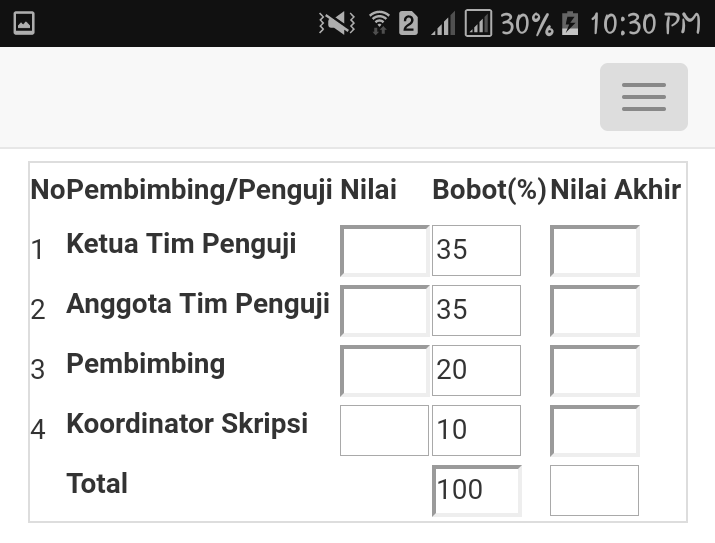
\includegraphics[scale=0.2]{Gambar/hp_nilai}
	\caption{Tampilan lembar nilai berita acara sidang skripsi sistem pada platform browser smartphone}
	\label{fig:hp_nilai}
\end{figure}

\begin{figure}[H]
	\centering
	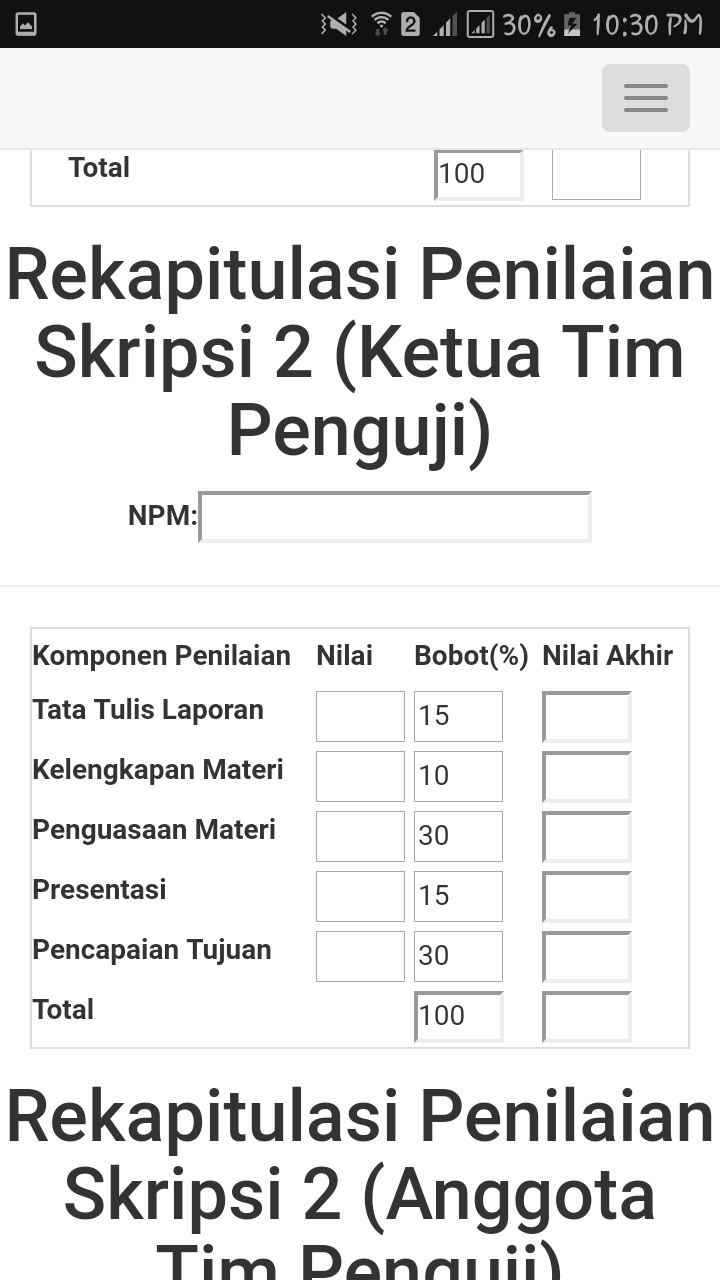
\includegraphics[scale=0.2]{Gambar/hp_ketua}
	\caption{Tampilan lembar rekapitulasi ketua tim penguji sistem pada platform browser smartphone}
	\label{fig:hp_ketua}
\end{figure}

\begin{figure}[H]
	\centering
	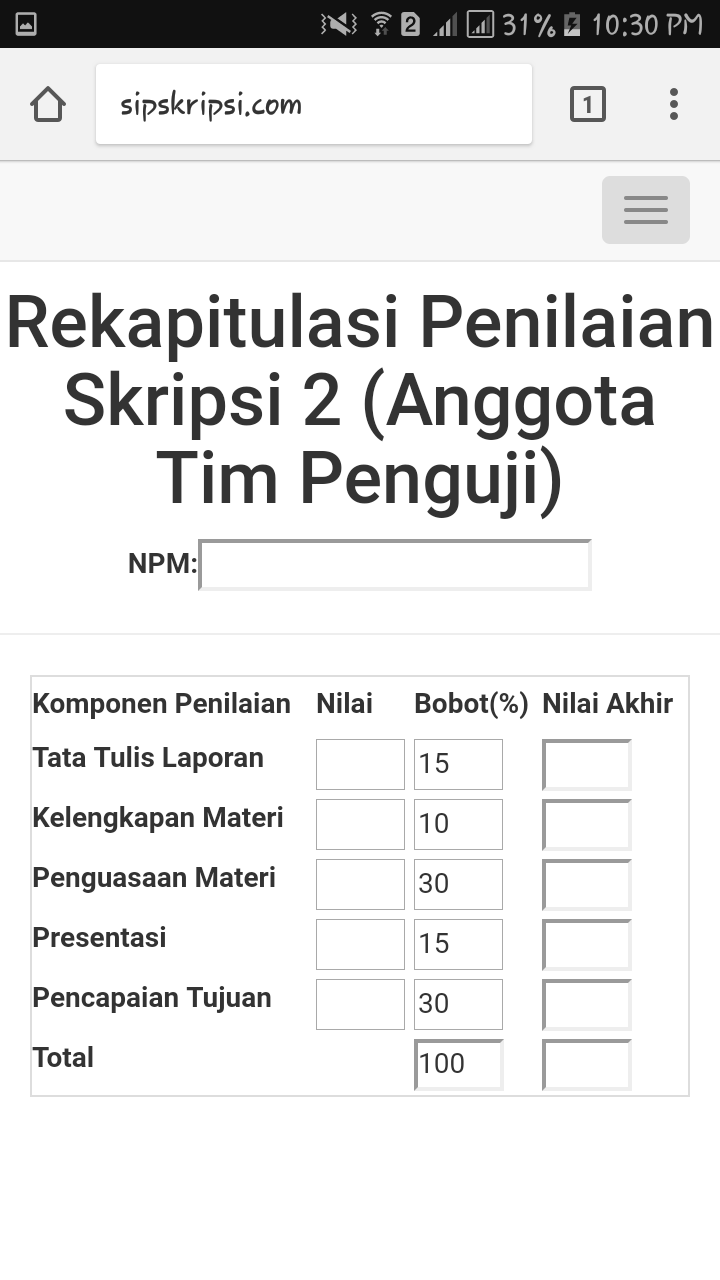
\includegraphics[scale=0.2]{Gambar/hp_anggota}
	\caption{Tampilan lembar rekapitulasi anggota tim penguji sistem pada platform browser smartphone}
	\label{fig:hp_anggota}
\end{figure}

\begin{figure}[H]
	\centering
	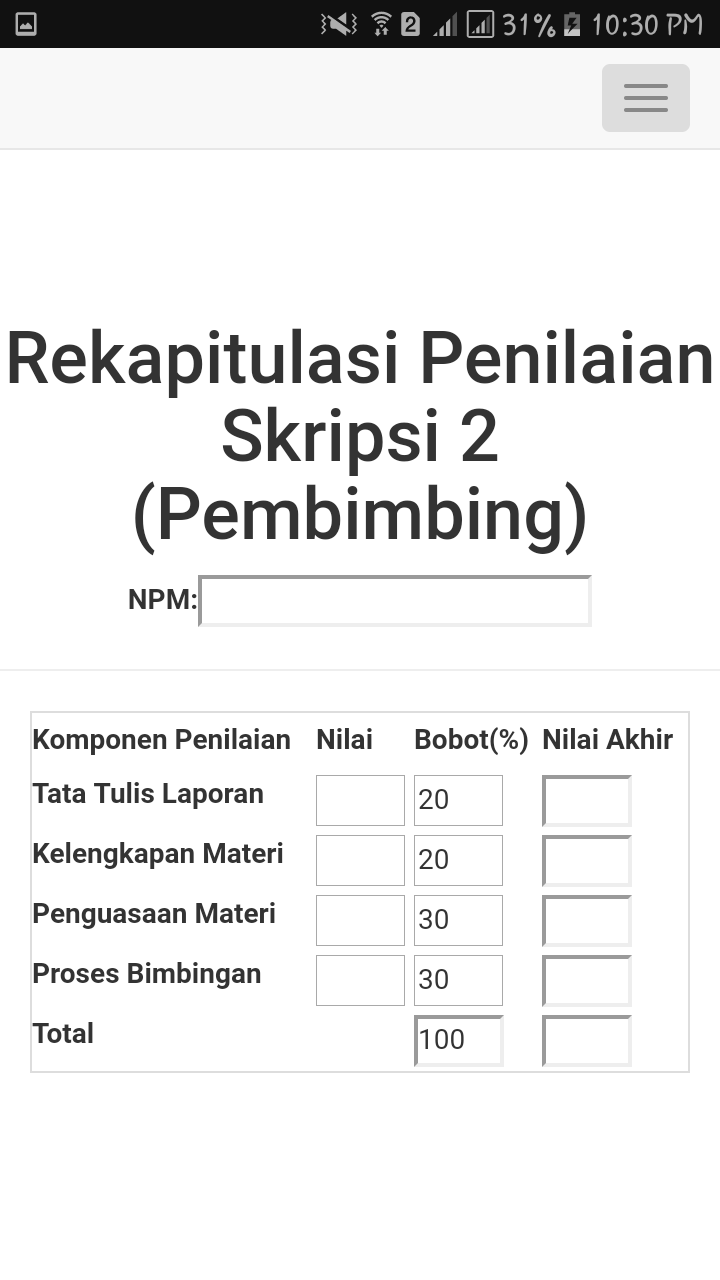
\includegraphics[scale=0.2]{Gambar/hp_pembimbing}
	\caption{Tampilan lembar rekapitulasi pembimbing sistem pada platform browser smartphone}
	\label{fig:hp_pembimbing}
\end{figure}

\begin{figure}[H]
	\centering
	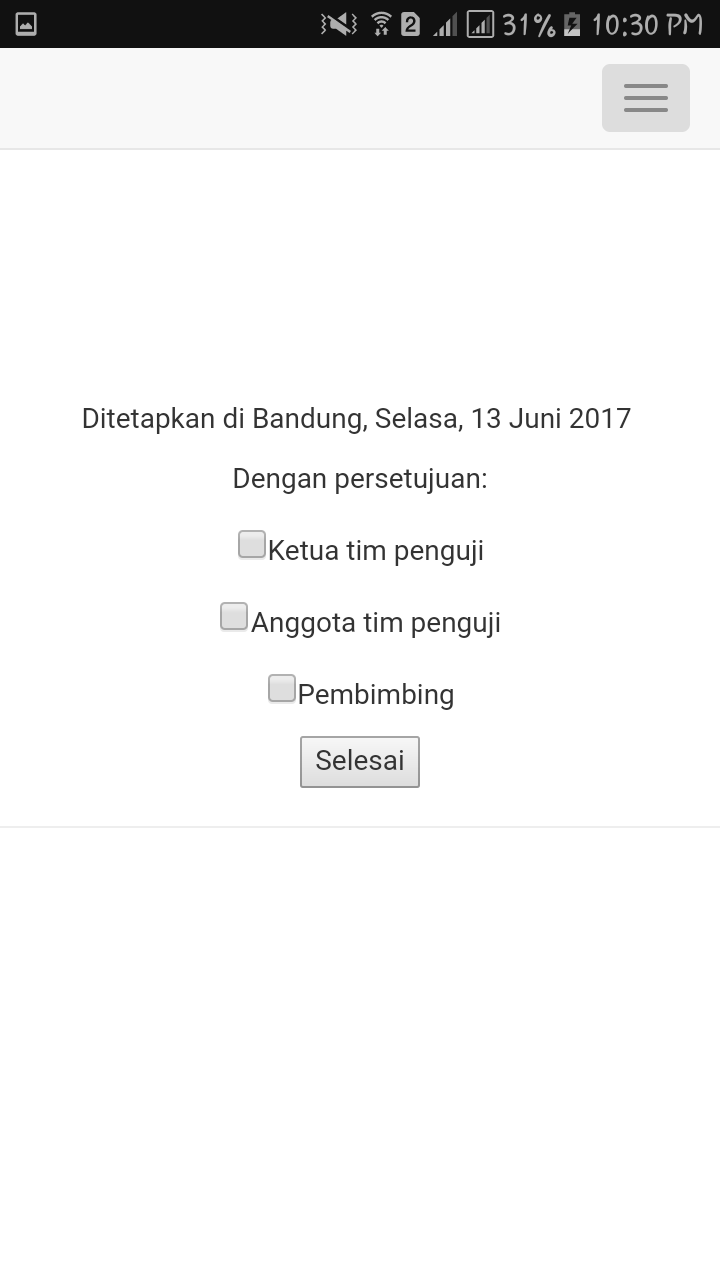
\includegraphics[scale=0.2]{Gambar/hp_selesai}
	\caption{Tampilan lembar selesai pada platform browser smartphone}
	\label{fig:hp_selesai}
\end{figure}